\documentclass{article}
\def\pgfsysdriver{pgfsys-tex4ht.def}
\usepackage{tikz}

% tikz setup for lattice graph
\usepackage{pgf}
\usetikzlibrary{automata}
\usetikzlibrary{positioning,chains,fit,shapes,calc}
\usetikzlibrary{arrows,shadows,trees}
\begin{document}
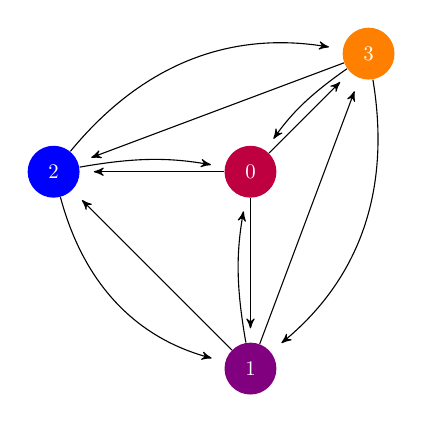
\begin{tikzpicture}[->,>=stealth',shorten >=5pt,auto,node distance=1cm]
            \tikzstyle{every state}=[fill=purple, draw=none,
            text=white]
            %                  D
            %      C      A 
            % 
            %             B
            \node[state, scale=0.75] (A) at (0,0)    {$0$};
            \node[state, scale=0.75, fill=violet] (B) at (0,-2.5)  {$1$};
            \node[state, scale=0.75, fill=blue] (C) at (-2.5,0) {$2$};
            \node[state, scale=0.75, fill=orange] (D) at (1.5,1.5) {$3$};
            \path (A) edge (B)% node {\scriptsize{Tr(0, -40)}} (B)
                  (A) edge (C) %node {\scriptsize{Tr(-40, 0)}} (C)
                  (A) edge (D); %node {\scriptsize{Tr(28,28)}}  (D);
            \path (B) edge [bend left=10] (A)
                  (B) edge (D) % node {\scriptsize{Tr(-40,0)}}  (D); 
                  (B) edge (C);% node {\scriptsize{Tr(-28,28)}} (C);
            \path (C) edge [bend right=30] (B)
                  (C) edge [bend left=10] (A)
                  (C) edge [bend left=30] (D);
            \path (D) edge [bend left=30] (B)
                  (D) edge [bend right=10] (A)
                  (D) edge (C);
                  
\end{tikzpicture}
\end{document}

 